\subsection*{Case Study}
The case-study used to explore this tools is the modelation made for the \textit{MWK (Manages With Knowledge)} project for the Software Systems Development subject during our graduation.

\begin{figure}[!htbp]
\begin{center}
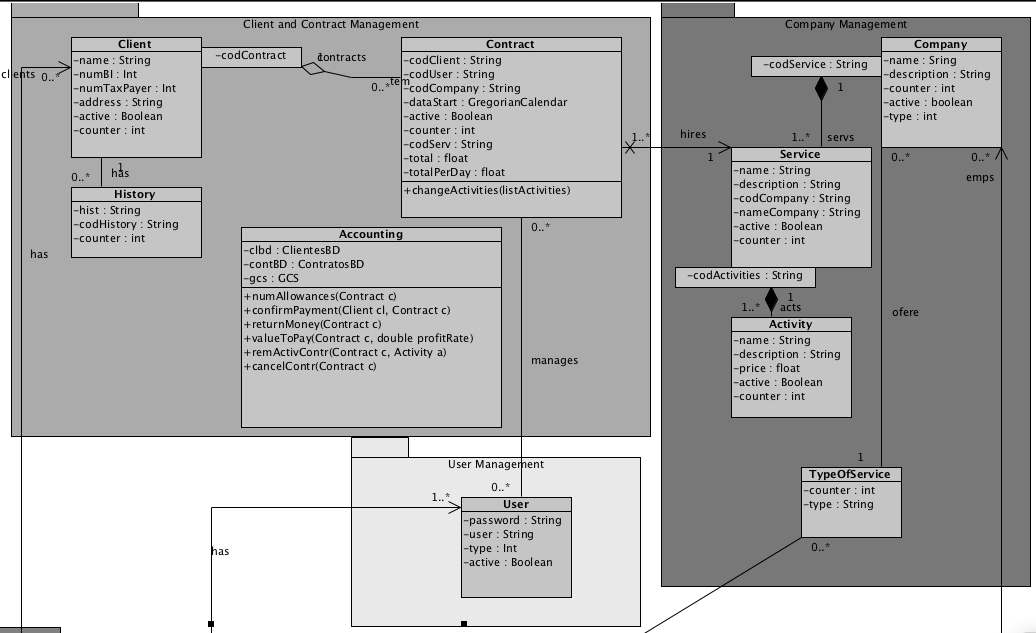
\includegraphics[scale=0.345]{images/classbw.png}
\caption{Excerpt of a Class diagram}\label{fig:class}
\end{center}
\end{figure} 

%\newpage
In this project, MWK is a company which does not provide services. 
In order to meet its clients needs it has a wide range of suppliers, that MWK subcontracts to be responsible for the service execution.
Multiple suppliers can supply the same service and each  service can be delivered in different ways.
Each service can then be composed of multiple activities. As an example, there could be a service called \textit{Shirts until 10 Kg} and inside this service there could be activities such as \textit{wash, iron, sewing buttons, etc}.
Each activity of a given service as a stipulated price, and can be hired by a client.
%The goal of the project was to model and implement a management software for this task.

\begin{figure}[!htbp]
\begin{center}
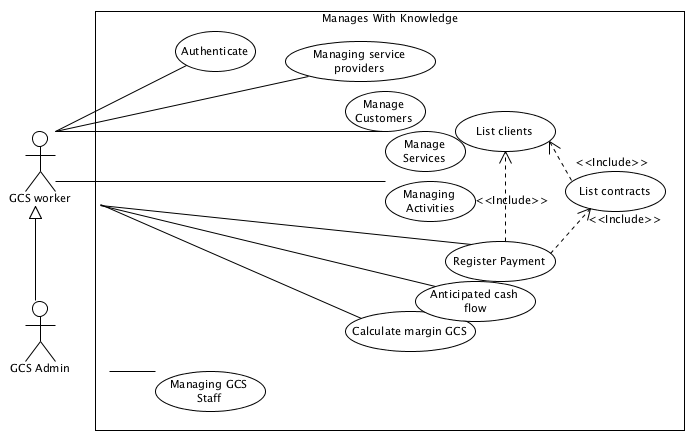
\includegraphics[width=0.9\textwidth]{images/usecase.png}
\caption{The general Use Case model}\label{fig:usecase}
\end{center}
\end{figure} 

As an example of the \uml\ diagrams used to model this task, we can see in Figure \ref{fig:usecase} an image of a general Use Case diagram and, in Figure \ref{fig:class}, an excerpt of a class diagram.
